\documentclass[../main.tex]{subfiles}

\begin{document}
\sloppy % Più permissivo nella gestione della giustificazione

% --- SOFTWARE ARCHITECTURE ---

\section{Software Architecture}\label{sec:software_architecture}

% --- DEPLOYMENT DIAGRAM ---

\subsection{Deployment Diagram}
The deployment diagram illustrates the distribution and interaction of the components within our dApp, highlighting how the system's parts connect and collaborate to deliver a functional application.

\begin{figure}[htbp]
    \centering
    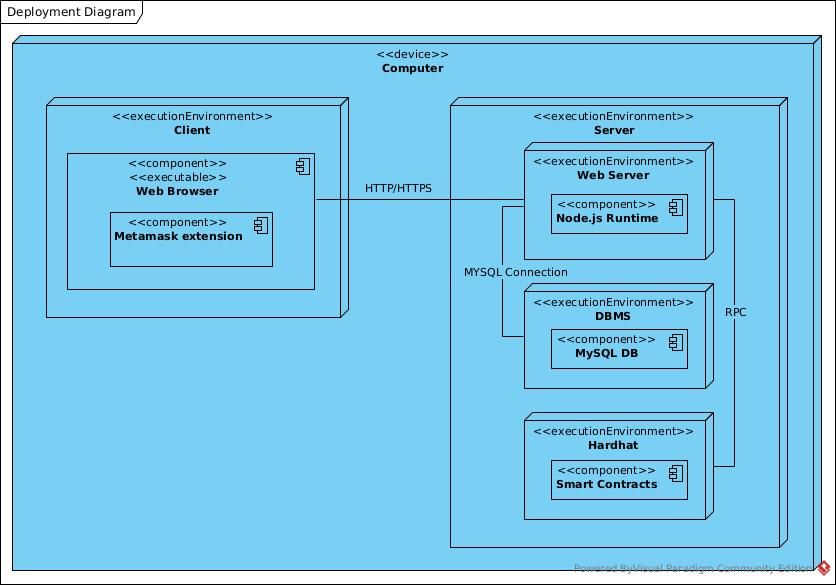
\includegraphics[width=\linewidth]{../src/diagrams/Deployment Diagram.jpg}
    \caption{dApp Deployment Diagram}
    \label{fig:deployDiag}
\end{figure}

The web application is developed using JavaScript with Handlebars for dynamic page rendering. It facilitates interaction with the blockchain via libraries like Web3.js and Ethers.js, while MetaMask is used to manage transactions and secure wallets.

On the backend, Node.js manages the server logic, while a MySQL database stores essential information, such as wallet-username associations and game scores. Blockchain interactions are handled via Hardhat, simplifying the deployment and testing of smart contracts that govern token management and score recording.

The architecture shown reflects the development environment, where all components run on a single machine, optimal for local testing but not indicative of the final production architecture.

% --- SMART CONTRACT CLASS DIAGRAM ---

\subsection{Smart Contract Class Diagram}
The smart contract manages the token economy of the dApp, handling token creation, distribution, and transfer. Below is the class diagram of the contract, outlining its core attributes and functions.

\begin{figure}[htbp]
    \centering
    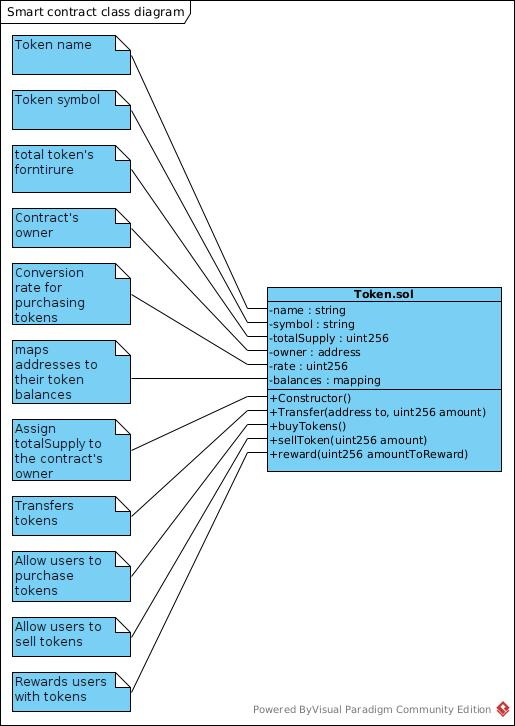
\includegraphics[width=0.5\textwidth]{../src/diagrams/Smart contract class diagram.jpg}
    \caption{Smart Contract Class Diagram}
    \label{fig:ClassDiag}
\end{figure}

The contract defines essential functions such as token transfers, purchases, and rewards. It manages user balances and token supply, while the `buyTokens` and `sellToken` functions handle the exchange between Ether and tokens. The `reward` function allows the contract owner to incentivize user participation.

% --- USE CASE DIAGRAM ---

\subsection{Use Case Diagram}
The following diagram outlines the key use cases for the Donuts Games dApp, including connecting a MetaMask wallet, playing minigames and quizzes, and managing Donuts (tokens).

\begin{figure}[H]
    \centering
    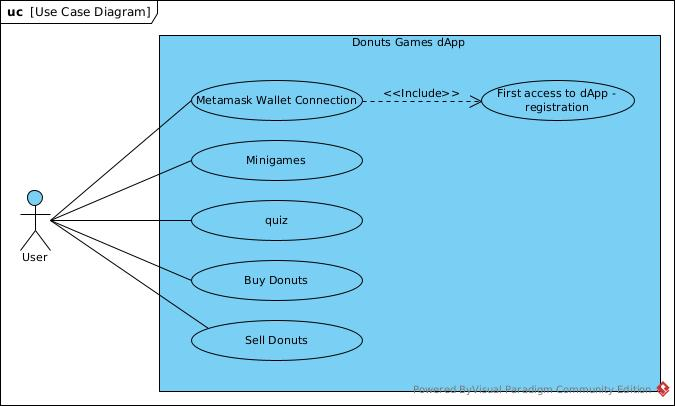
\includegraphics[width=\linewidth]{../src/diagrams/Use Case Diagram.jpg}
    \caption{dApp Use Case Diagram}
    \label{fig:useCaseDiag}
\end{figure}

Users start by connecting their MetaMask wallet, which also serves as a quick registration process for new users. They can then engage in various games, quizzes, and token management activities (buying and selling Donuts) through the smart contract.

The minigames use case generalizes the gameplay experiences across Minesweeper, Tetris, and Snake, providing users with different options for earning tokens while playing. Similarly, the quiz use case generalizes the available quizzes on Blockchain, Smart Contracts, and Ethereum, offering a range of educational content that allows users to earn tokens based on their knowledge.

% --- SEQUENCE DIAGRAMS ---

\subsection{Sequence Diagrams}
The sequence diagrams illustrate the interaction between the user's wallet, frontend, backend, and smart contracts during key user actions, each corresponding to the use cases previously described.

% --- WALLET CONNECTION SEQUENCE DIAGRAM ---

\subsubsection{Wallet Connection Sequence Diagram}

\begin{figure}[H]
    \centering
    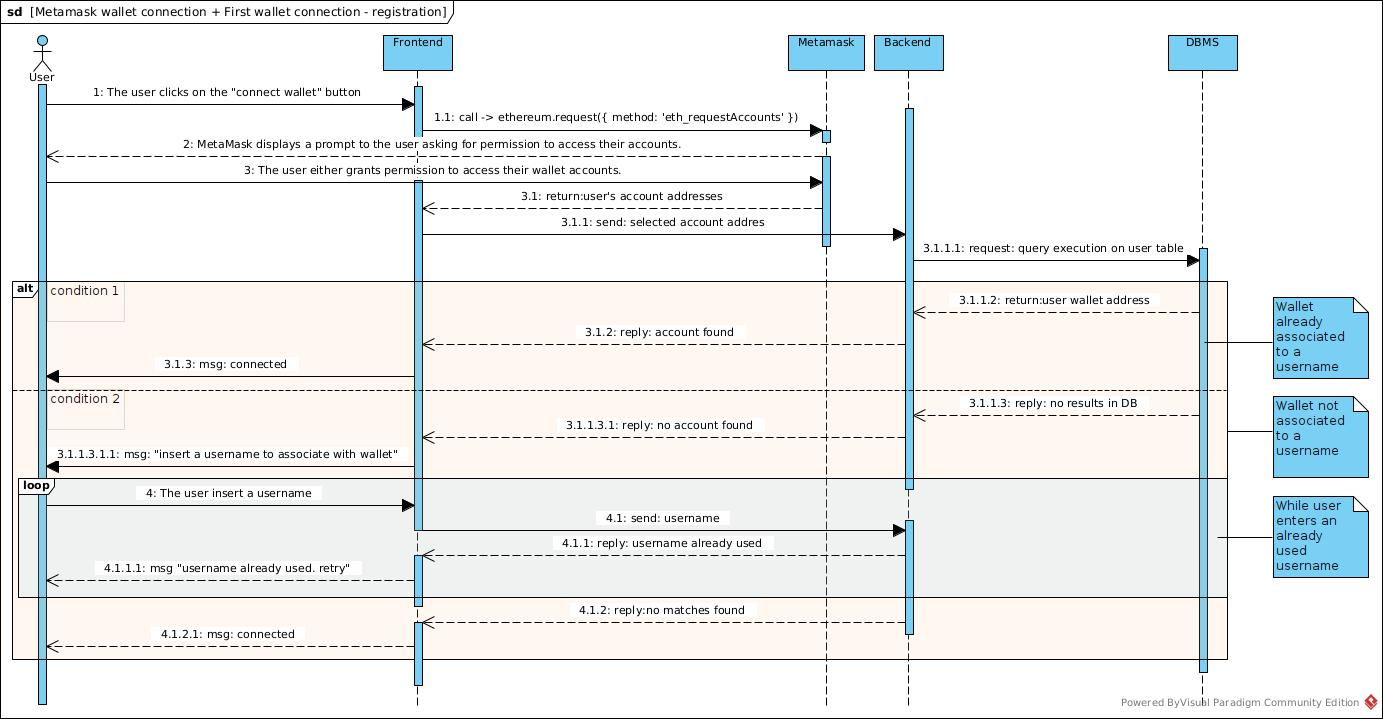
\includegraphics[width=\linewidth]{../src/diagrams/Metamask wallet connection + First wallet connection - registration.jpg}
    \caption{Wallet connection sequence diagram}
    \label{fig:walletConn_seqDiag}
\end{figure}

This diagram shows the process of connecting a MetaMask wallet, either associating it with an existing username or creating a new profile if not previously registered. Error handling for duplicate usernames is included.

% --- MINIGAMES SEQUENCE DIAGRAM ---

\subsubsection{Minigames Sequence Diagram}

\begin{figure}[H]
    \centering
    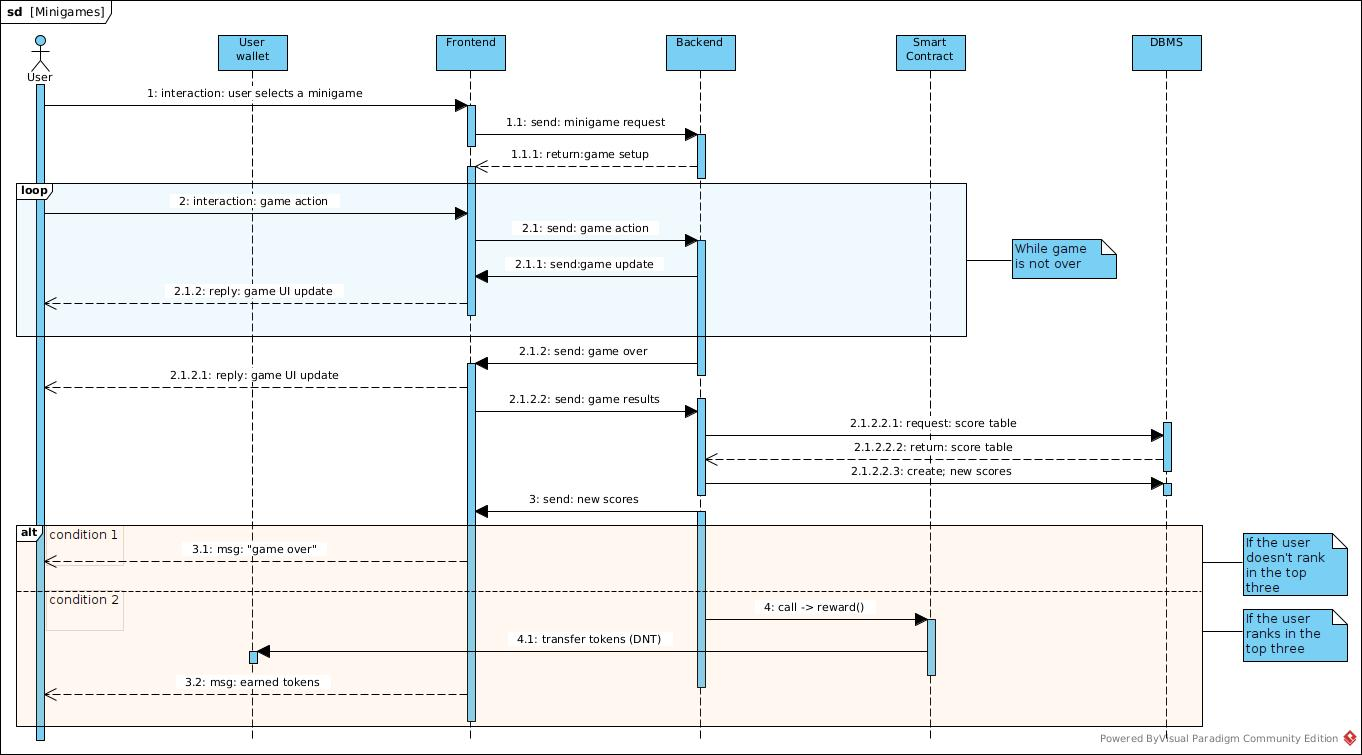
\includegraphics[width=\linewidth]{../src/diagrams/Minigames.jpg}
    \caption{Minigames sequence diagram}
    \label{fig:Minigames_seqDiag}
\end{figure}

This diagram illustrates how users engage with minigames, showing interactions between the frontend, backend, and smart contract during gameplay. Since the minigames (Tetris, Minesweeper, and Snake) share the same mechanics, they are generalized into a single use case.

% --- QUIZ SEQUENCE DIAGRAM ---

\subsubsection{Quiz Sequence Diagram}

\begin{figure}[H]
    \centering
    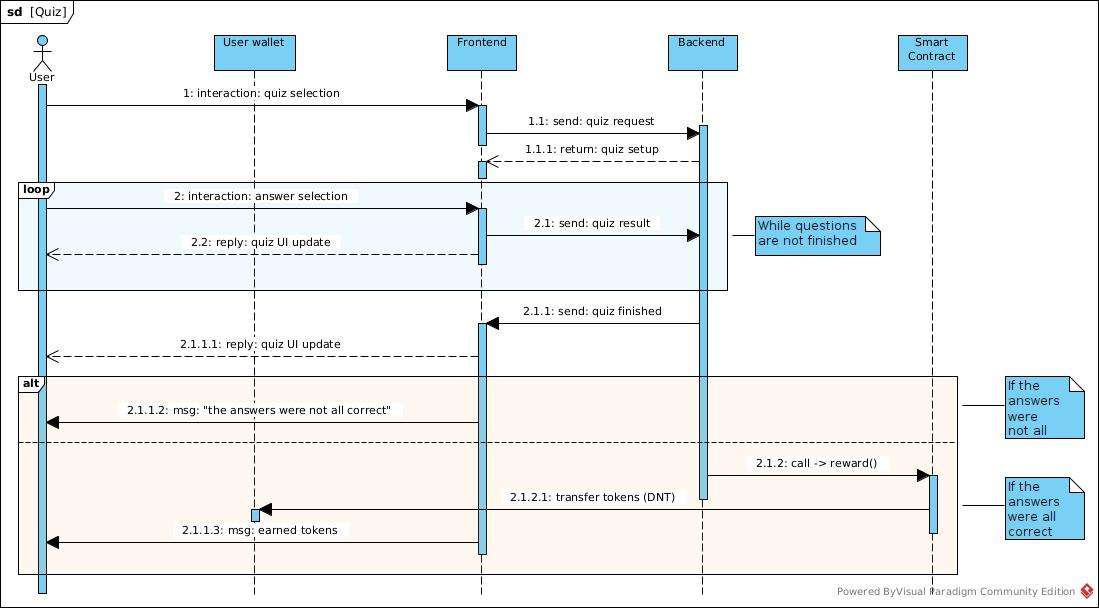
\includegraphics[width=\linewidth]{../src/diagrams/Quiz.jpg}
    \caption{Quiz sequence diagram}
    \label{fig:Quiz_seqDiag}
\end{figure}

This diagram shows the flow when users participate in quizzes. The frontend and backend present quiz questions, validate answers, and issue rewards based on correctness. The quizzes (Blockchain, Smart Contracts, and Ethereum) are generalized due to their shared structure.

% --- BUY DONUTS SEQUENCE DIAGRAM ---

\subsubsection{Buy Donuts Sequence Diagram}

\begin{figure}[H]
    \centering
    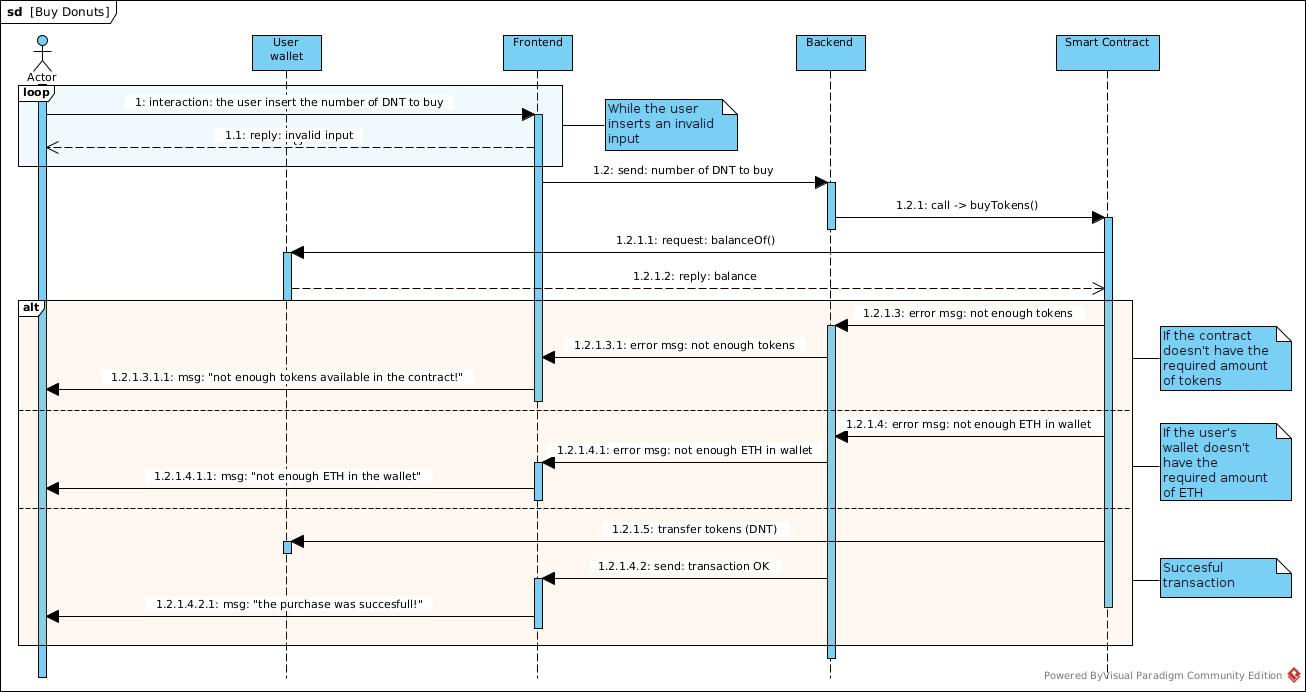
\includegraphics[width=\linewidth]{../src/diagrams/Buy Donuts.jpg}
    \caption{Buy Donuts sequence diagram}
    \label{fig:buyDNT_seqDiag}
\end{figure}

This diagram outlines the process of buying DNT tokens, verifying whether the user has enough ETH and if the contract has sufficient tokens. Error handling for insufficient funds or tokens is included.

% --- SELL DONUTS SEQUENCE DIAGRAM ---

\subsubsection{Sell Donuts Sequence Diagram}

\begin{figure}[H]
    \centering
    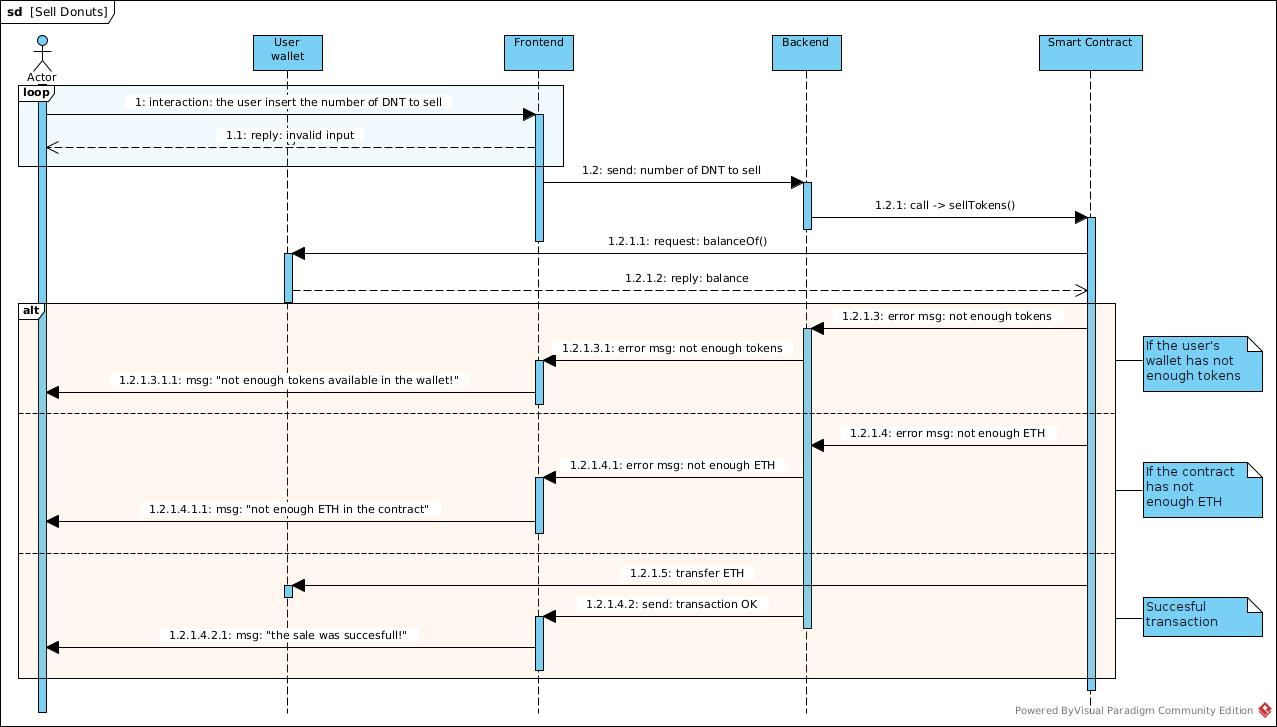
\includegraphics[width=\linewidth]{../src/diagrams/Sell Donuts.jpg}
    \caption{Sell Donuts sequence diagram}
    \label{fig:sellDNT_seqDiag}
\end{figure}

This diagram shows the process of selling DNT tokens, including balance validation and the availability of ETH for payout. Error handling for insufficient tokens or ETH is also covered.

\end{document}

% \documentclass[../main.tex]{subfiles}

% \begin{document}
% \sloppy % Più permissivo nella gestione della giustificazione

% % --- SOFTWARE ARCHITECTURE ---

% \section{Software Architecture}\label{sec:software_architecture}

% % --- DEPLOYMENT DIAGRAM ---

% \subsection{Deployment Diagram}
% \sloppypar
% The deployment diagram provides an overview of the distribution and interaction of the components within our decentralized application (dApp). This visual representation is crucial for understanding how the different parts of the system connect and collaborate to deliver a functional and cohesive application.
% \justifying
% \begin{figure}[htbp] % Posizionamento dell'immagine
%     \centering % Centra l'immagine orizzontalmente
%     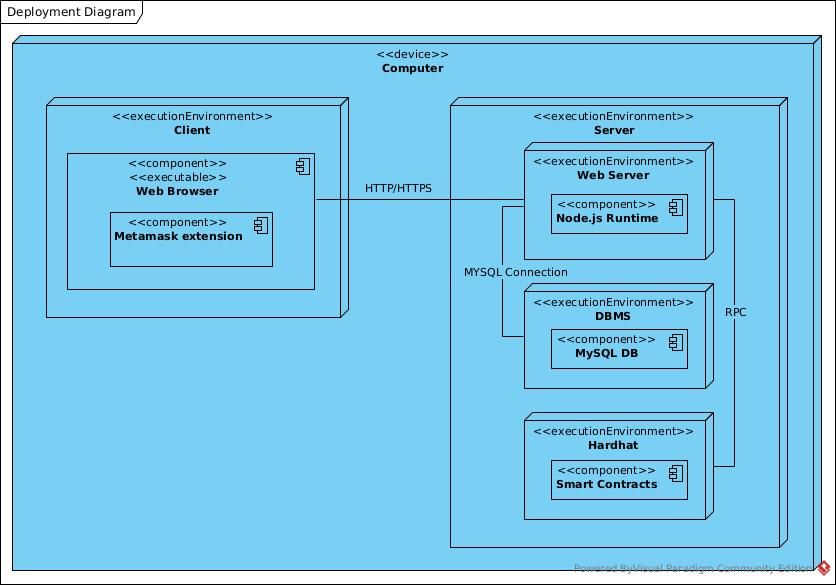
\includegraphics[width=\linewidth]{../src/diagrams/Deployment Diagram.jpg} % Imposta la larghezza dell'immagine alla larghezza massima disponibile
%     \caption{dApp Deployment Diagram} % Didascalia dell'immagine
%     \label{fig:deployDiag} % Etichetta per i riferimenti incrociati
% \end{figure}

% The web application is developed in JavaScript using Handlebars (hbs) for dynamic page rendering, allowing users to interact through a simple and intuitive interface. Interactions with the blockchain are managed through libraries like Web3.js or Ethers.js, which facilitate communication with smart contracts. Users manage transactions and their Ethereum wallets via MetaMask, a browser extension that ensures secure handling of private keys and transactions.

% The user’s browser, equipped with MetaMask, communicates with the server via HTTP/HTTPS, ensuring secure data exchange. MetaMask allows users to manage private keys and approve transactions required for interactions with smart contracts on the Ethereum network.

% As for the server side, the backend uses Node.js as the runtime environment to manage server-side logic and handle requests from the client. The server is connected to a MySQL database, which stores essential information such as the association between Ethereum wallets and usernames, as well as game scores. The MySQL database is managed through phpMyAdmin, and the connection between the web server and the database is established through a MySQL connection, ensuring efficient and secure data exchange.

% For blockchain interactions, we use Hardhat, a development environment for Ethereum that simplifies the deployment and testing of smart contracts. The smart contracts implemented on the Ethereum blockchain handle essential functions such as managing the platform’s tokens (DNT) and recording game scores. The connection between Hardhat and the web server is established via RPC (Remote Procedure Call) communications, allowing the server to interact with the blockchain as if the operations were executed locally, simplifying the execution of remote operations on the smart contracts.

% It is important to note that the architecture depicted in the diagram reflects the development environment, where all components — server, database, and blockchain development environment — run on a single machine. This configuration is optimal for local testing and development but does not reflect the final production architecture, which could involve distributed resources and cloud services to ensure scalability and availability in a real-world context.

% % --- COMPONENT DIAGRAM ---

% \subsection{Components Diagram}
% xxx

% % --- SMART CONTRACT CLASS DIAGRAM ---

% \subsection{Smart Contract Class Diagram}
% The following section presents the design and functionality of the smart contract that governs the token economy within our dApp. This contract, written in Solidity and deployed on the Ethereum blockchain, is responsible for managing the creation, distribution, and transfer of tokens. The diagram below outlines the core attributes and functions of the contract, providing a structured view of the token’s functionality and behavior.

% Below is the class diagram of the smart contract, detailing its internal structure, key components, and the flow of operations, including purchasing, selling, transferring tokens, and rewarding users.

% \begin{figure}[htbp] % Posizionamento dell'immagine
%     \centering % Centra l'immagine orizzontalmente
%     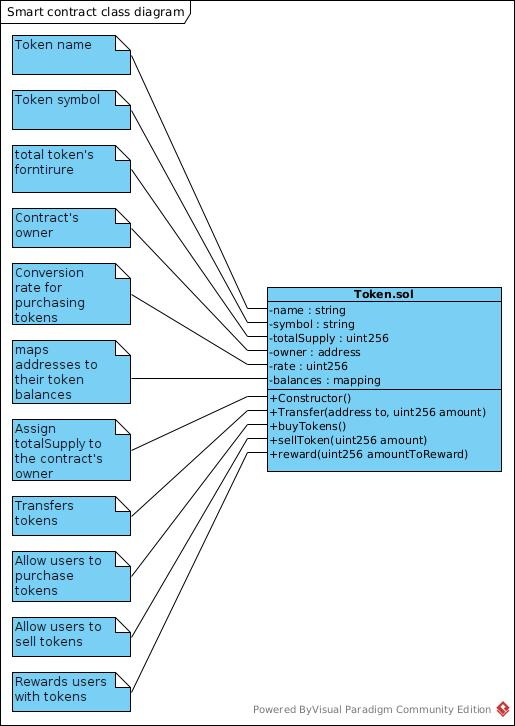
\includegraphics[width=0.5\textwidth]{../src/diagrams/Smart contract class diagram.jpg} % Imposta la larghezza dell'immagine al 50% della larghezza del testo
%     \caption{Smart Contract Class Diagram} % Didascalia dell'immagine
%     \label{fig:ClassDiag} % Etichetta per i riferimenti incrociati
% \end{figure}

% The smart contract represented by the class Token.sol is at the core of our token economy, defining how tokens are created, managed, and interacted with on the blockchain. It lays out the essential functions that govern the distribution, transfer, and purchasing of tokens by users.

% At the foundation of the contract are the token's name and symbol, both stored as strings. These attributes give the token its identity on the blockchain and remain constant once the contract is deployed, ensuring consistency across the system.

% The total supply of tokens is represented by the variable totalSupply, which is of type uint256. This variable defines the total number of tokens that will ever exist, and its value is set when the contract is deployed. This mechanism ensures a finite supply, limiting the number of tokens that can be distributed.

% Ownership of the contract is managed by the owner variable, which stores the Ethereum address of the contract’s creator. The owner has certain administrative privileges within the contract, such as the ability to distribute tokens or modify certain parameters. This structure ensures that there is a central figure responsible for the management of the contract’s operations.

% A key feature of the contract is the conversion rate for purchasing tokens, stored in the rate variable. This rate, defined as a uint256, determines how many tokens a user receives in exchange for a certain amount of Ether. It’s an essential component for managing the token economy and ensuring a fair exchange system.

% The contract also maintains a mapping of each user’s Ethereum address to their token balance through the balances variable. This structure ensures that the contract keeps track of how many tokens each user owns, enabling the system to manage transfers and validate balances.

% When the contract is first initialized, the constructor function plays a critical role. It assigns the total token supply to the owner and sets the initial values for key attributes such as the token's name, symbol, total supply, and conversion rate. This step ensures that the contract is properly set up before users can interact with it.

% One of the core functionalities of the contract is the transfer function, which allows tokens to be sent from one user to another. This function takes two parameters: the recipient’s address and the amount of tokens to transfer. It enables the free movement of tokens within the ecosystem, making the token tradable between users.

% The contract also includes a buyTokens function, which allows users to purchase tokens by sending Ether to the contract. Based on the conversion rate, the contract calculates how many tokens the user is entitled to and credits their account accordingly. This function provides a straightforward way for users to acquire tokens.

% In addition to buying tokens, users can also sell them back to the contract using the sellToken function. This allows them to exchange their tokens for Ether at the defined conversion rate. The contract calculates the amount of Ether to be returned to the user and transfers it back to them, enabling a fluid exchange between tokens and Ether.

% Lastly, the contract includes a reward function, which allows the owner to distribute tokens as rewards. This can be used as an incentive mechanism within the dApp, where users can be rewarded for certain behaviors or achievements. By transferring tokens directly to a user’s account, the reward system helps drive engagement and participation in the platform.

% % --- USE CASE DIAGRAM ---

% \subsection{Use Case Diagram}
% The following diagram illustrates the key use cases for the Donuts Games dApp. It provides a visual representation of how users interact with the various features of the application. The diagram outlines the core functionalities available to users, including connecting their MetaMask wallet, playing minigames and quizzes, as well as buying and selling donuts (tokens within the dApp).

% \begin{figure}[H] % Forza l'immagine a essere inserita subito dopo il testo
%     \centering % Centra l'immagine orizzontalmente
%     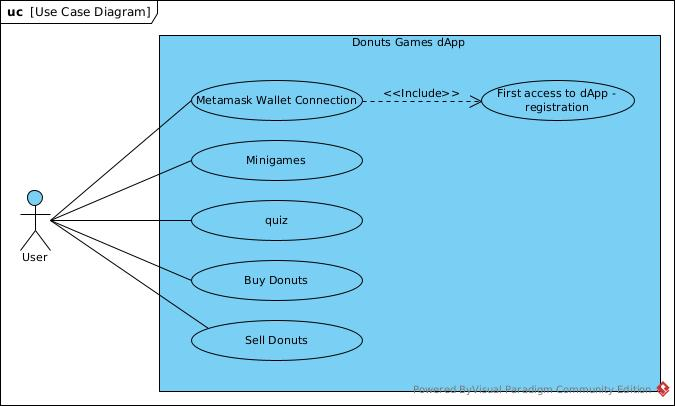
\includegraphics[width=\linewidth]{../src/diagrams/Use Case Diagram.jpg} % Imposta la larghezza dell'immagine alla larghezza massima disponibile
%     \caption{dApp Use Case Diagram} % Didascalia dell'immagine
%     \label{fig:useCaseDiag} % Etichetta per i riferimenti incrociati
% \end{figure}

% The MetaMask Wallet Connection is the user’s first interaction with the Donuts Games dApp, enabling secure linking of their Ethereum wallet to unlock the platform's blockchain features. For new users, this step also includes a quick registration that stores their wallet details and creates a profile, ensuring future interactions are secure and personalized.

% Once connected, users can dive into minigames, which offer both entertainment and rewards through engagement with the dApp's token economy. These games make participation fun while allowing users to earn tokens.

% The quiz feature adds another dimension, letting users test their knowledge and earn tokens based on performance. This feature combines entertainment with tangible rewards in the tokenized system.

% Users can also buy Donuts, the dApp's native token, using Ether. The smart contract ensures a secure, real-time transaction that updates the user's token balance. With these tokens, users can fully engage with the platform’s economy.

% For those looking to convert tokens back into Ether, the Sell Donuts feature provides an easy, two-way exchange, offering liquidity and flexibility in their interactions with the platform.

% % --- SEQUENCE DIAGRAM ---

% \subsection{Sequence Diagrams}
% In this section, we present the sequence diagrams that outline the interaction between different components of the Donuts Games dApp. Each diagram corresponds to a use case described in the previous section, providing a detailed view of how the system's components interact during key user actions.

% The sequence diagrams illustrate the flow of communication between the user's wallet, the frontend, the backend, and the smart contract or database management system (DBMS), depending on the context. These diagrams highlight the essential steps in each use case, including checks for validity, error handling, and successful outcomes.

% % --- WALLET CONNECTION SEQUENCE DIAGRAM ---

% \subsubsection{Wallet Connection Sequence Diagram}

% \begin{figure}[H] % Forza l'immagine a essere inserita subito dopo il testo
%     \centering % Centra l'immagine orizzontalmente
%     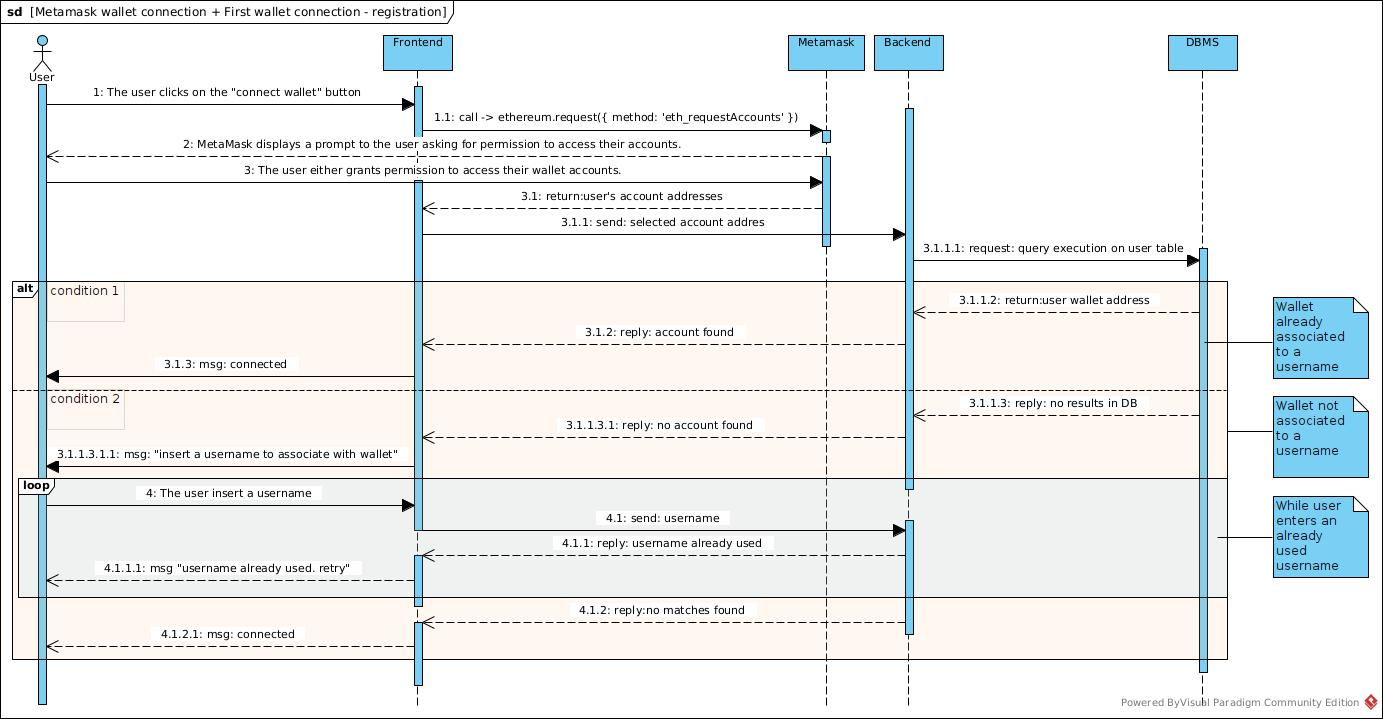
\includegraphics[width=\linewidth]{../src/diagrams/Metamask wallet connection + First wallet connection - registration.jpg} % Imposta la larghezza dell'immagine alla larghezza massima disponibile
%     \caption{Wallet connection sequence diagram} % Didascalia dell'immagine
%     \label{fig:walletConn_seqDiag} % Etichetta per i riferimenti incrociati
% \end{figure}

% This diagram depicts the user's initial interaction with the Donuts Games dApp when connecting their MetaMask wallet. It covers scenarios such as account association with an existing username or creating a new profile if the wallet has not been previously registered. Error handling for duplicate usernames is also displayed.

% % --- MINIGAMES SEQUENCE DIAGRAM ---

% \subsubsection{Minigames Sequence Diagram}

% \begin{figure}[H] % Forza l'immagine a essere inserita subito dopo il testo
%     \centering % Centra l'immagine orizzontalmente
%     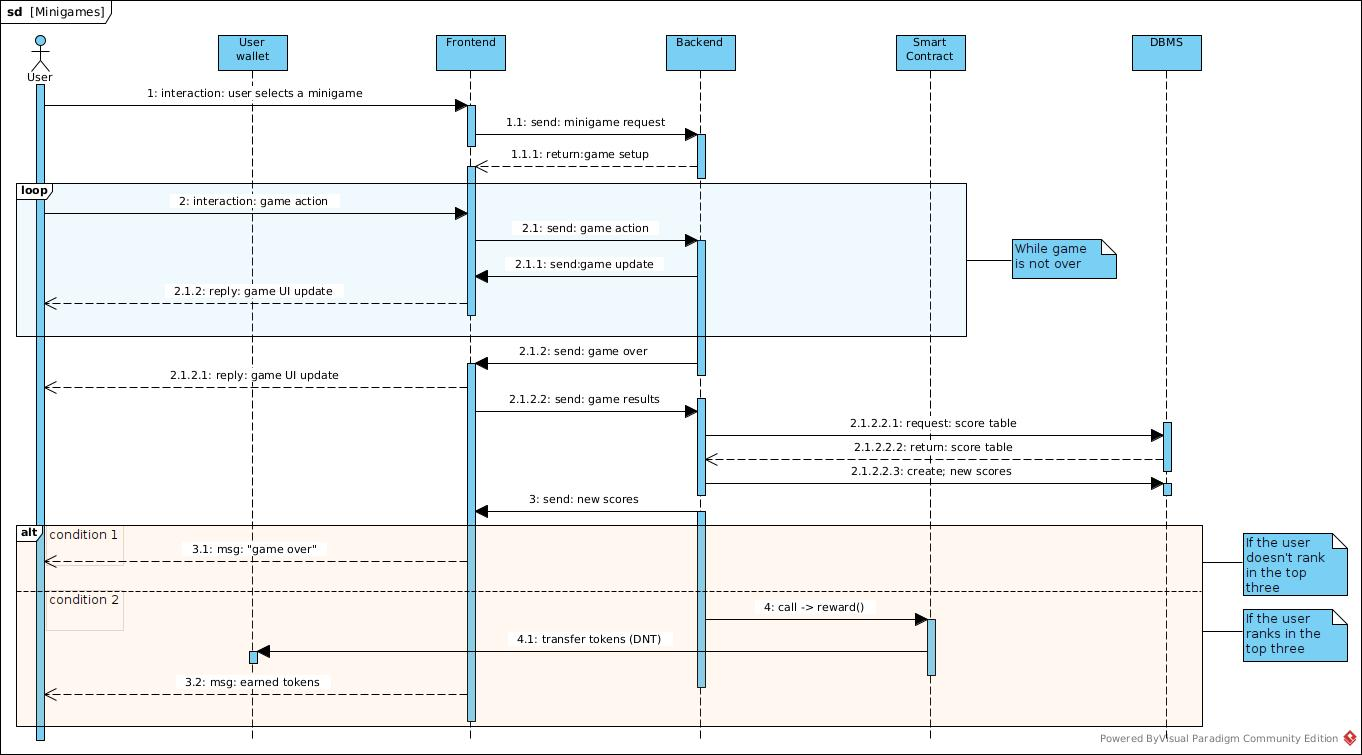
\includegraphics[width=\linewidth]{../src/diagrams/Minigames.jpg} % Imposta la larghezza dell'immagine alla larghezza massima disponibile
%     \caption{Minigames sequence diagram} % Didascalia dell'immagine
%     \label{fig:Minigames_seqDiag} % Etichetta per i riferimenti incrociati
% \end{figure}

% The sequence diagram for this use case illustrates how users can engage in a minigame within the dApp. It outlines the interactions between the frontend, backend, and smart contract during gameplay, including updating the game state, recording scores, and rewarding users with tokens based on their performance. Since the three minigames available (Tetris, Minesweeper, and Snake) share the same underlying mechanics, they have been generalized into a single use case.

% % --- QUIZ SEQUENCE DIAGRAM ---

% \subsubsection{Quiz Sequence Diagram}

% \begin{figure}[H] % Forza l'immagine a essere inserita subito dopo il testo
%     \centering % Centra l'immagine orizzontalmente
%     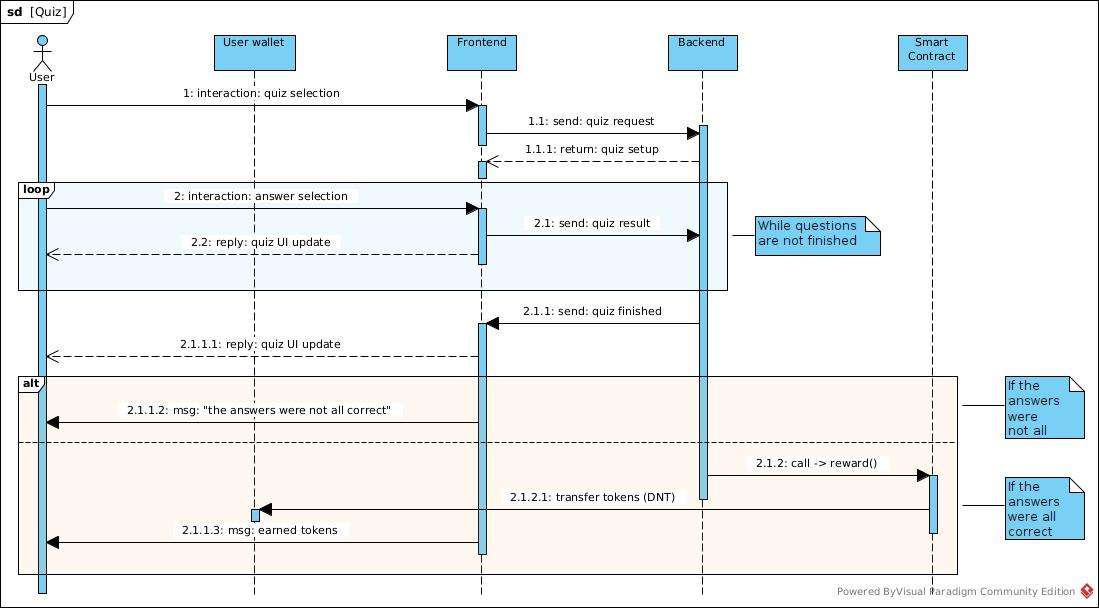
\includegraphics[width=\linewidth]{../src/diagrams/Quiz.jpg} % Imposta la larghezza dell'immagine alla larghezza massima disponibile
%     \caption{Quiz sequence diagram} % Didascalia dell'immagine
%     \label{fig:Quiz_seqDiag} % Etichetta per i riferimenti incrociati
% \end{figure}

% This diagram shows the flow when users participate in a quiz. It details how the frontend and backend interact to present the quiz questions, validate the user's answers, and determine if rewards in the form of tokens should be issued based on the correctness of the responses. Since the three available quizzes (Blockchain, Smart Contracts, and Ethereum) share the same structure and logic, they have been generalized into a single use case.

% % --- BUY DONUTS SEQUENCE DIAGRAM ---

% \subsubsection{Buy Donuts Sequence Diagram}

% \begin{figure}[H] % Forza l'immagine a essere inserita subito dopo il testo
%     \centering % Centra l'immagine orizzontalmente
%     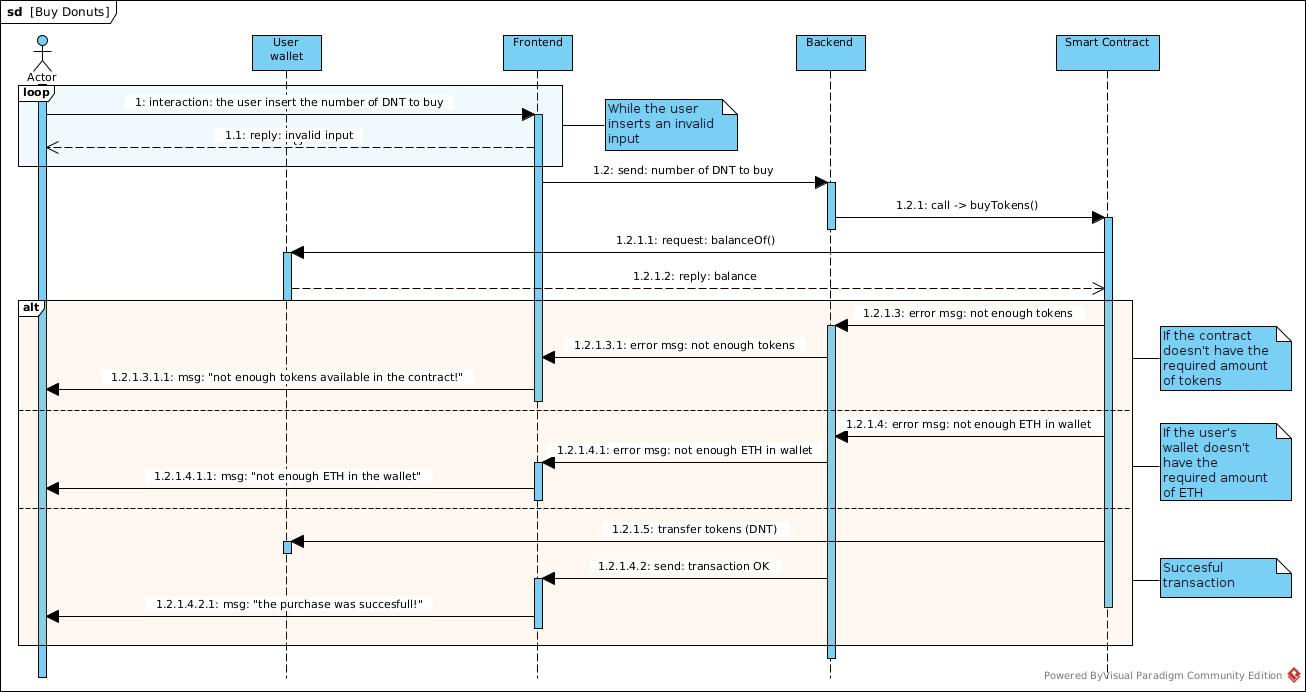
\includegraphics[width=\linewidth]{../src/diagrams/Buy Donuts.jpg} % Imposta la larghezza dell'immagine alla larghezza massima disponibile
%     \caption{Buy Donuts sequence diagram} % Didascalia dell'immagine
%     \label{fig:buyDNT_seqDiag} % Etichetta per i riferimenti incrociati
% \end{figure}

% This diagram details the process of purchasing the native token, DNT. It shows the interaction between the user, the backend, and the smart contract to verify if the user has enough Ethereum (ETH) to buy the tokens and whether the smart contract has enough tokens available. Different scenarios are handled, such as insufficient ETH or tokens, leading to error messages, while a successful transaction results in a token transfer.

% % --- SELL DONUTS SEQUENCE DIAGRAM ---

% \subsubsection{Sell Donuts Sequence Diagram}

% \begin{figure}[H] % Forza l'immagine a essere inserita subito dopo il testo
%     \centering % Centra l'immagine orizzontalmente
%     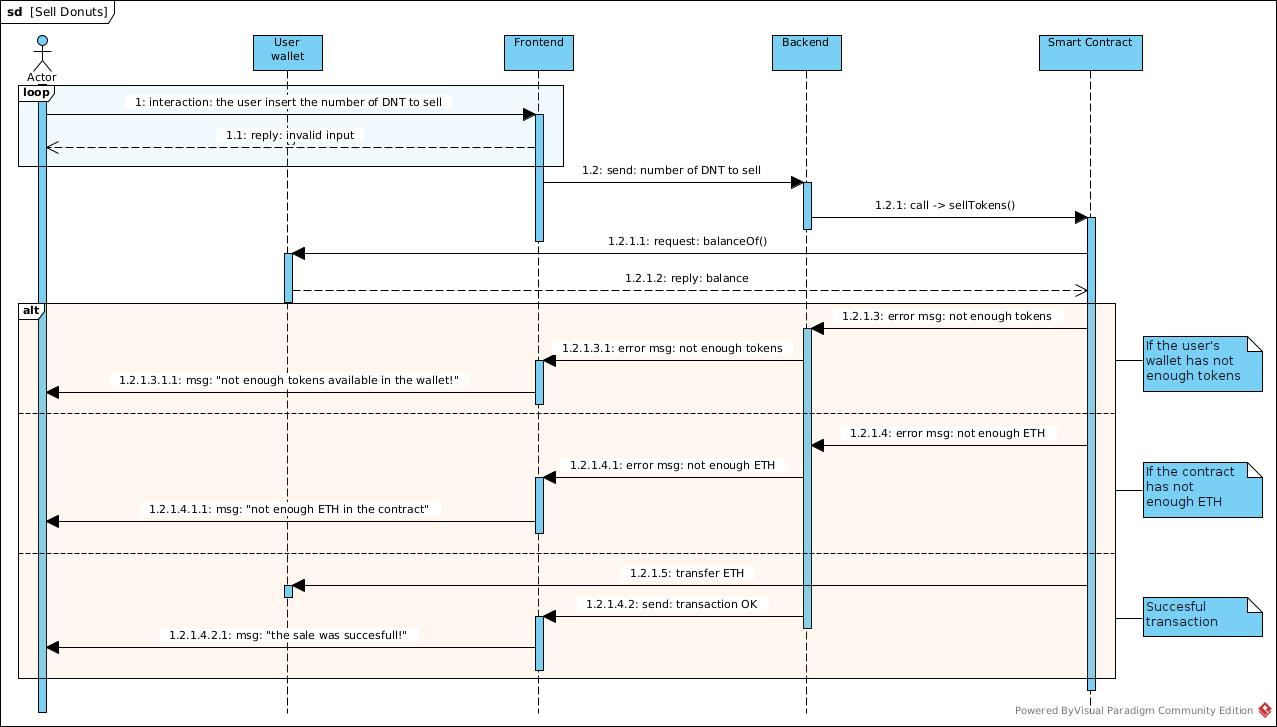
\includegraphics[width=\linewidth]{../src/diagrams/Sell Donuts.jpg} % Imposta la larghezza dell'immagine alla larghezza massima disponibile
%     \caption{Sell Donuts sequence diagram} % Didascalia dell'immagine
%     \label{fig:sellDNT_seqDiag} % Etichetta per i riferimenti incrociati
% \end{figure}

% This sequence diagram describes the process of selling DNT tokens. It captures the validation of the user's balance, the availability of ETH in the smart contract for payout, and the steps to complete the transaction. Similar to the buy process, error handling for insufficient funds or tokens is clearly outlined.
% \end{document}


